% chapter 4 section 4

\section{电磁感应}

\subsection{电磁感应}

\subsubsection{楞次定律}

\begin{figure}[ht!]
    \centering
    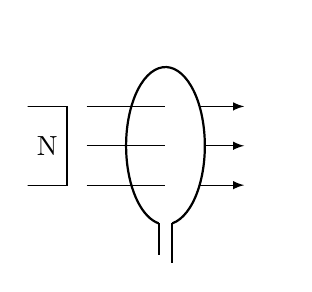
\begin{tikzpicture}[scale=0.5]
        \clip (-3.5,-3) rectangle (3,3);
        \draw (-4,-1) rectangle (-2.5,1);
        \node at (-3,0) {N};
        \foreach \y in {-1,0,1} \draw[-latex] (0,\y) -- (2,\y);
        \filldraw[thick, draw=black, fill=white] (-80:1 and 2) arc (-80:260:1 and 2);
        \draw[thick] (-80:1 and 2) -- ++ (0,-1);
        \draw[thick] (260:1 and 2) -- ++ (0,-0.8);
        \foreach \y in {-1,0,1} \draw (-2,\y) -- (0,\y);
    \end{tikzpicture}
    \caption{楞次定律}
\end{figure}
实验表明磁场的变化会激发出相应的电的效果,即电磁感应现象,日文为電磁誘導。其中称激发出来的电流为感应电流(誘導電流),称与之对应的起电力为感应电势(誘導起電力)。描述其感应电流方向的定律为楞次定律,日文为レンツの法則。
\begin{itembox}[l]{楞次定律}
    \centering
    变化的磁场会产生妨碍该变化的感应电流/电势(增反减同)
\end{itembox}

\subsubsection{法拉第电磁感应定律}

日文为ファラデーの電磁誘導の法則,其定量地描述了磁生电的效果。为此我们需要率先明确磁通量的概念。

磁通量,日文为磁束,是描述给定面上磁场大小的量,一般用字母$\Phi$表示。应注意只有与给定面垂直的部分才会被计为磁通量。
\begin{equation*}
    \Phi=B\cdot S
\end{equation*}

至此,磁生电的现象则可由磁通量随时间的变化描述,即法拉第电磁感应定律。
\begin{equation*}
    V=-\frac{\Delta\Phi}{\Delta t}
\end{equation*}

\subsubsection{运动导体的感应电势}

\paragraph{一般模型}实际题目中常常很难直接使用法拉第电磁感应定律,而是更多使用其在特定模型下的形式。题目中常见的模型如下,空间中布满匀强磁场,平行金属导轨上有一根可移动的金属棒,让金属棒以一定速度运动,探究此时的感应电势。
\begin{figure}[ht!]
    \centering
    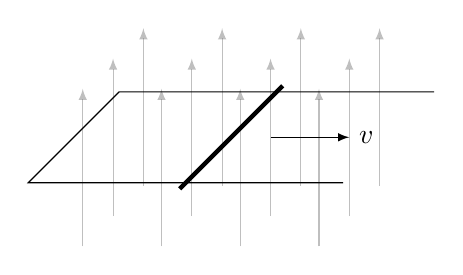
\begin{tikzpicture}
        \foreach \x in {0.5,1.5,2.5,3.5} \foreach \z in {0.5,1.5,2.5}
            \draw[-latex,color=gray,opacity=0.5] (\x,-1,\z) -- (\x,1,\z);
        \draw (4,0,0) -- (0,0,0) -- (0,0,3) -- (4,0,3);
        \draw[ultra thick] (2,0,-0.2) -- (2,0,3.2);
        \draw[-latex] (2.5,0,1.5) -- (3.5,0,1.5) node[right] {$v$};
    \end{tikzpicture}
    \caption{电磁感应水平模型}
\end{figure}
根据法拉第电磁感应定律可得感应电势大小为
\begin{equation*}
    |V|=\frac{\Delta\Phi}{\Delta t}=\frac{BS}{t}=\frac{B\Delta xl}{\Delta t}=Bvl
\end{equation*}
其方向可由楞次定律或者右手定则判断。
\begin{itemize}
    \item 磁场穿过手心
    \item 拇指与运动方向同向
    \item 四指为电流方向
\end{itemize}

\paragraph{斜面模型}时而题目中会出现斜向的平行导轨。
\begin{figure}[ht!]
    \centering
    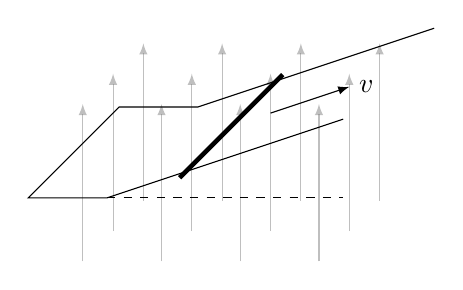
\begin{tikzpicture}
        \foreach \x in {0.5,1.5,2.5,3.5} \foreach \z in {0.5,1.5,2.5}
            \draw[-latex,color=gray,opacity=0.5] (\x,-1,\z) -- (\x,1,\z);
        \draw (4,1,0) -- (1,0,0) -- (0,0,0) -- (0,0,3) -- (1,0,3) -- (4,1,3);
        \draw[dashed] (1,0,3) -- (4,0,3);
        \drawangle{(4,0,3)}{(1,0,3)}{(4,1,3)};
        \draw[ultra thick] (2,1/3,-0.2) -- (2,1/3,3.2);
        \draw[-latex] (2.5,0.5,1.5) -- (3.5,5/6,1.5) node[right] {$v$};
    \end{tikzpicture}
    \caption{电磁感应斜面模型}
\end{figure}
此时实际与金属棒运动方向垂直的磁通量密度为$B\cos\theta$,根据磁通量的定义可得
\begin{equation*}
    V=Bvl\cos\theta
\end{equation*}

\paragraph{圆环模型}此外题目中偶尔也会出现稍复杂一些的圆环模型。
\begin{figure}[ht!]
    \centering
    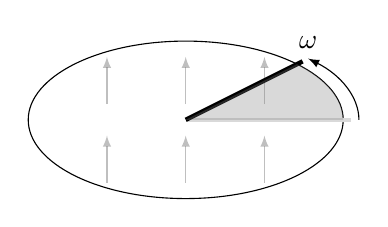
\begin{tikzpicture}
        \foreach \x in {-1,0,1} \foreach \y in {-0.5,0.5}
            \draw[-latex,color=gray,opacity=0.5] (\x,{\y-0.3}) -- (\x,{\y+0.3});
        \draw (0,0) circle (2 and 1);
        \draw[ultra thick, color=gray!30] (0,0) --(2.1,0);
        \draw[ultra thick] (0,0) -- (45:2.1 and 1.05);
        \draw[-latex] (2.2,0) arc (0:45:2.2 and 1.1) node[above] {$\omega$};
        \fill[color=gray,opacity=0.3] (0,0) -- (2,0) arc (0:45:2 and 1) --cycle;
    \end{tikzpicture}
    \caption{电磁感应圆环模型}
\end{figure}
根据扇形公式可知,在$\Delta t$的时间内金属棒会扫过$\Delta S=\frac12\omega\Delta tl^2$的面积,结合法拉第电磁感应定律可得
\begin{equation*}
    V=\frac12\omega Bl^2
\end{equation*}

\subsubsection{自感与互感}

\textbackslash\textbackslash TODO

\subsection{交流电}

\textbackslash\textbackslash TODO
